%\section{Adding in Between Chains of the Same Period}

\Cref{fig:minrep.adding1.overview} shows both the periods of the model initially, as described in \Cref{chap:minrep}, as well as the model with period-adding structures.
For \Cref{fig:minrep.adding1.overview.adding}, only the values of the fixed parameters $a_L = 1, b_L = 0.5$ are changed.
Initially, the values for these parameters were $a_L = 4, b_L = -0.5$.
The only other fixed parameter $B$ stays the same and the parameter ranges of $p_x$ and $p_y$ are adjusted slightly in order to get the same bifurcation phenomena.
That means, that the shape of the function only changed on the branches $f_{\A}$ and $f_{\C}$.

When comparing both figures, we can see that there are no ``type B'' period regions in \Cref{fig:minrep.adding1.overview.adding}, the period-adding situation.
Instead, it looks like the ``type A'' period regions of the same period overlap now.
Also, the regions of higher periods in between the chains are new, these are the period-adding regions.
At the points, where these regions make a turn, there are parameter regions of even higher periods.
The meaning of this will be explored in a later section, the next section will focus on the nature of the period adding structures.
%The meaning of these is explored in a later section, the next section will focus on the disappearance of the ``type B'' parameter regions.
\todo{reference later section concerned with corners}

\begin{figure}
    \centering
    \subfloat[Initial situation]{
        \includegraphics[width=.5 \textwidth]{62_MinimalRepr_Adding/2D_Period_4/result.png}
        \label{fig:minrep.adding1.overview.initial}
    }
    \subfloat[Period-adding]{
        \includegraphics[width=.5 \textwidth]{62_MinimalRepr_Adding/2D_Period_1/result.png}
        \label{fig:minrep.adding1.overview.adding}
    }
    \caption{Overview of period-adding structures in between chains of the same period}
    \label{fig:minrep.adding1.overview}
\end{figure}

\section{Changes on the Path to Period-adding}

\begin{enumerate}
    \item \begin{itemize}
              \item ``type A'' parameter regions stop overlapping with the ``type A'' period regions above them (lower period, same number of points on branches $f_\B$ and $f_\D$)
              \item Point where boundaries cross. On the left: no overlap, period-adding. On the right: overlap
              \item This point moves right until no overlap exists anymore
          \end{itemize}
    \item \begin{itemize}
              \item ``type A'' parameter regions start overlapping with the ``type A'' period regions above right them (same period)
              \item Point where boundaries cross. On the left: overlap. On the right: no overlap, ``type B'' parameter region
              \item This point moves right, until no ``type B'' parameter region exists anymore
          \end{itemize}
    \item \begin{itemize}
              \item ``type A'' parameter regions stop overlapping with the ``type A'' parameter regions right to them (higher period, one more point on branches $f_\B$ and $f_\D$)
              \item This seems to happen in an instant
          \end{itemize}
\end{enumerate}

Timeline:
On the parameter line outlined above, the processes happen as follows.
First, the process (i) starts.
While it is happening, the process (ii) starts and finishes, before (i) finishes.
Lastly the process (iii) starts and finishes directly.
After all that, process (i) is the last to complete.

\subsection{Disappearance of ``Type B'' Parameter Regions}
\label{sec:minrep.adding.disapp.typeB}

\todo{small intro, then another subsubsection}

\Cref{fig:minrep.path.to.disappearance} shows diagrams depicting the borders of parameter regions of specific stable cycles.
The lower left corner of the diagrams is always in the period region with the stable cycle $P_{10}^3 \equiv \Cycle{\A^7\B^3\C^7\D^3}$, the cycles in the upper left ($\Cycle{\A^6\B^3\C^6\D^3}$), upper right ($\Cycle{\A^6\B^4\C^6\D^4}$), lower right ($\Cycle{\A^7\B^4\C^7\D^4}$), and middle ($\Cycle{\A^7\B^3\C^6\D^4}$ and $\Cycle{\A^6\B^4\C^7\D^3}$) follow.
\todo{always short form / always long form / both?}
The diagrams show the evolution of the ``type B'' parameter region along a line in the parameter space from \Cref{fig:minrep.adding1.overview.initial} ($a_L = 4, b_L = -0.5$) to \Cref{fig:minrep.adding1.overview.initial} $a_L = 1, b_L = 0.5$.
This line is given by the equation $a_L = \frac{5}{2} - 3 \cdot b_L$.

\Cref{fig:minrep.path.to.disappearance.1} shows the first change that occurs on this path to period-adding.
The ``type A'' parameter region $P_{11}^4$ does no longer overlap with the ``type A'' parameter region $P_{10}^4$.
This happens to all parameter regions $P_{x}^y$, they do no longer overlap with the parameter region $P_{x-1}^y$.
But this is only true for the left side of their overlap.
On the right side they still do overlap, as we can see from the parameter regions $P_{10}^3$ and $P_{9}1^3$ in \Cref{fig:minrep.path.to.disappearance.1}.
All other overlaps remain, but they are a lot smaller now, especially the overlaps of the ``type B'' parameter region $Q_{10}^3$ in the middle with the surrounding ``type A'' parameter regions.
In the space between the lower and upper right ``type A'' parameter regions, period adding emerges.

In the next diagram, \Cref{fig:minrep.path.to.disappearance.2}, the parameter region $P_{10}^3$ now overlaps with the parameter region $P_{10}^4$.
The new overlapping area pushes the ``type B'' parameter region to the side.
It is now smaller and only has 3 boundaries.

This overlap is completed in \Cref{fig:minrep.path.to.disappearance.3} and the ``type B'' parameter region disappears completely.
In \Cref{fig:minrep.path.to.disappearance.3}, the ``type B'' parameter region is completely replaced by the overlapping ``type A'' parameter regions $P_{10}^3$ and $P_{10}^4$.
Also the ``type A'' parameter regions $P_9^3$ and $P_{10}^4$ do not overlap anymore.
The same is true for the ``type A'' parameter regions $P_{10}^3$ and $P_{11}^4$ and we can conclude it is for all $P_x^y$ and $P_{x+1}^{y+1}$.

\Cref{fig:minrep.path.to.disappearance.3} shows the parameter region boundaries when the process is completed.
The last overlap of the ``type A'' parameter regions $P_{10}^3$ and $P_{9}^3$, and therefore all $P_x^y$ and $P_{x+1}^y$, is gone.
Only the ``type A'' parameter regions with the same period overlap and in between the ``type A'' parameter regions with different periods, there is period adding.


\begin{figure}
    \centering
    \subfloat[$a_L = 2.8, b_L = -0.1$]{
        \includegraphics[width=.5 \textwidth]{62_MinimalRepr_Adding/2D_Regions_2.8/Manual/result.png}
        \label{fig:minrep.path.to.disappearance.1}
    }
    \subfloat[$a_L = 2.725, b_L = -0.075$]{
        \includegraphics[width=.5 \textwidth]{62_MinimalRepr_Adding/2D_Regions_2.725/Manual/result.png}
        \label{fig:minrep.path.to.disappearance.2}
    } \\
    \subfloat[$a_L = 2.65, b_L = -0.05$]{
        \includegraphics[width=.5 \textwidth]{62_MinimalRepr_Adding/2D_Regions_2.65/Manual/result.png}
        \label{fig:minrep.path.to.disappearance.3}
    }
    \subfloat[$a_L = 2.5, b_L = 0$]{
        \includegraphics[width=.5 \textwidth]{62_MinimalRepr_Adding/2D_Regions_2.5/Manual/result.png}
        \label{fig:minrep.path.to.disappearance.4}
    }
    \caption{Evolution of ``type B'' parameter regions when transitioning to a period adding scenario}
    \label{fig:minrep.path.to.disappearance}
\end{figure}

\subsubsection{``Type B'' Cycles Just Before Disappearing}

Just before the ``type B'' period region disappears, at $a_L = 2.675, b_L = -0.58\overline{3}$, the cycles that exist there are extremely close to colliding with 3 different borders each.
\Cref{fig:minrep.just.before.disappearance.cobb} shows the cobweb diagram of the cycles.
Both cycles are so close to each other on branches $f_\A$ and $f_\B$, that we can't tell them apart.
Even in the vastly enhanced blowup plot in the upper left corner of the figure, both cycles are almost on top of each other.
At the boundary $d_1$ the cycles split, because of the symmetry the same happens at $d_3$ again.
At $d_1$, the cycle $\Cycle{\A^7\B^3\C^6\D^4}$ (green) is mapped onto $f_\A$ one last time, while its twin cycle $\Cycle{\A^6\B^4\C^7\D^3}$ (brown) is directly mapped to $f_\B$.
At $d_3$, the same thing happens, but the two cycles are swapped.

As for the cycles near $d_0$ and $d_2$, the cycle $\Cycle{\A^7\B^3\C^6\D^4}$ is next to $d_2$, while its twin cycle is near $d_0$.
The collision of the cycles with the borders at the same time corresponds to the right boundary of the ``type B'' period region.
This follows from \Cref{sec:minrep.bif}, where all bifurcations in this model are listed and explained.
The two bifurcations are denoted as $\BCB_{d_0}^{\A^6\B^4\C^7\D^3, r}$ and $\BCB_{d_2}^{\A^7\B^3\C^6\D^4, r}$.
As this boundary does not move as much as the other two still existing boundaries when transitioning to the period adding scenario, this bifurcation is not as important to us now.

The cycles near $d_1$ and $d_3$ correspond to the upper and lower boundaries of the ``type B'' period region.
Again, the correspondence follows from \Cref{sec:minrep.bif}.
The upper and lower boundaries of ``type B'' period regions are border collision bifurcations where the two cycles collide with $d_1$ and $d_3$ at the same time, one cycle with one boundary each.
For the upper boundary, the cycle with more points on the branch $f_\A$ collides with the border $d_3$ from the left, denoted as $\BCB_{d_3}^{\A^7\B^3\C^6\D^4, l}$.
Its twin cycle collides with $d_1$, also from the left.
This follows from the symmetry and is denoted as $\BCB_{d_1}^{\A^6\B^4\C^7\D^3, l}$.
For the lower boundary, now the cycles collide from the right instead of the left, but the borders with which each cycle collides stay the same.
So for this boundary we have the bifurcations $\BCB_{d_3}^{\A^7\B^3\C^6\D^4, l}$ and $\BCB_{d_1}^{\A^6\B^4\C^7\D^3, r}$.
These two boundaries get closer to each other as we lower $a_L$ as we can see in \Cref{sec:minrep.adding.disapp.typeB}.

\begin{figure}
    \centering
    \subfloat[Regions]{
        \includegraphics[width=.3 \textwidth]{62_MinimalRepr_Adding/2D_Regions_2.675/Manual/result.png}
        \label{fig:minrep.just.before.disappearance.reg}
    }
    \subfloat[Cobweb at point $A$]{
        \includegraphics[width=.3 \textwidth]{62_MinimalRepr_Adding/Cob_2.675_A/Manual/result.png}
        \label{fig:minrep.just.before.disappearance.coba}
    }
    \subfloat[Cobweb at point $B$]{
        \includegraphics[width=.3 \textwidth]{62_MinimalRepr_Adding/Cob_2.675_B/Manual/result.png}
        \label{fig:minrep.just.before.disappearance.cobb}
    }
    \label{fig:minrep.just.before.disappearance}
    \caption{Disappearance of the ``type B'' parameter region}
\end{figure}

To see what happens after the boundaries of the ``type B'' period region crossed each other, we take a look at point $A$.
\Cref{fig:minrep.just.before.disappearance.coba} shows the cobweb diagram at this point.
The two cycles that exist here look similar to the cycles in \Cref{fig:minrep.just.before.disappearance.cobb}, they have a similar number of points on each branch.
Also, two cycles are near borders $d_1$ and $d_3$, one on the left and one on the right, as well as one cycle being near $d_0$ and $d_2$.
But with this cobweb diagram, the basins of attraction on the right half are not the inverse of the basins of attraction on the left half, but the same.
This hints at the fact that we are now dealing with ``type A'' cycles that are symmetric.

\todo{order of left most cycle and other cycle => type B or type A}

\todo{parallels to next appearing period adding}
\subsection{Appearance of Period Adding}

\subsubsection{Horizontal}

\begin{figure}
    \centering
    \subfloat[Regions]{
        \includegraphics[width=.3 \textwidth]{62_MinimalRepr_Adding/2D_Regions_2.8_add_hor/Manual/result.png}
    }
    \subfloat[At point $A$]{
        \includegraphics[width=.3 \textwidth]{62_MinimalRepr_Adding/Cob_2.8_add_hor_A/Manual/result.png}
        \label{fig:minrep.add.app.hor.A}
    }
    \subfloat[At point $B$ \todo{replace figure}]{
        \includegraphics[width=.3 \textwidth]{62_MinimalRepr_Adding/Cob_2.8_add_hor_A/Manual/result.png}
        \label{fig:minrep.add.app.hor.B}
    }
    \caption{Appearance of the horizontal period-adding cascade}
\end{figure}

At point $A$ there is space between the two ``type A'' parameter regions $P_{11}^{4}$ and $P_{10}^{4}$, which overlap at point $B$.
This space opens up more as we change the parameters as described in \Cref{sec:minrep.adding.disapp.typeB}.
Here will be the horizontal period adding region.
\Cref{fig:minrep.add.app.hor.A} shows the cobweb diagram at this point.
The two coexisting cycles $\Cycle{\A^7\B^4\C^6\D^4}$ and $\Cycle{\A^6\B^4\C^7\D^4}$ are asymmetrical like in ``type B'' parameter regions.
But they are different from ``type B'' cycles because they are not of the form $\Cycle{\A^a\B^b\C^{a-1}\D^{b+1}}$ and $\Cycle{\A^{a-1}\B^{b+1}\C^a\D^b}$, but of the form $\Cycle{\A^a\B^b\C^{a-1}\D^b}$ and $\Cycle{\A^{a-1}\B^b\C^a\D^b}$.

If we interpret these cycles in the context of the halved model, this is the first stage of the period-adding cascade.
The two ``type A'' cycles $P_{11}^4$ and $P_{10}^4$ are $\Cycle{\L^7\R^4}$ and $\Cycle{\L^6\R^4}$ in the context of the halved model and the cycles at point $A$ are both $\Cycle{\L^7\R^4\L^6\R^4} \equiv \Cycle{\L^6\R^4\L^7\R^4}$ in the context of the halved model.

In \Cref{sec:minrep.adding.disapp.typeB} we noted, that the asymmetry of the ``type B'' cycles is caused by the negative slope of the function at the left border of branches $f_\A$ and $f_\C$.
Since this maps the cycle that starts further left to the right side of the other cycle.
\todo{
    explain better: diff number of points on branches B and D each (type B) therefore reordering necessary for asymm.
    type b also: split at $d_1, d_3$ as well as $d_2$ and $d_0$, here only $d_1, d_3$ (two boundaries).
    here same number of points so there must be no reordering for asymm
}
This is not the case for the cycles at this point, both cycles start at a point on the branch $f_\A$ with a positive slope and therefore keep the same order.
\todo{positive slope important for period adding!}

\begin{figure}
    \centering
    \includegraphics[width=.7 \textwidth]{62_MinimalRepr_Adding/1D_Bif_2.8_add_hor_AU/Manual/result.png}
    \caption{Bifurcation diagram at the upper boundary of $P_{10}^4 \oplus P_{11}^4$}
    \label{fig:minrep.add.app.hor.bif.AU}
\end{figure}


\Cref{fig:minrep.add.app.hor.bif.AU} show the bifurcations at the top of the parameter region of the first period-adding stage.
The bifurcation of the ``type A'' cycle $P_{10}^4 \equiv \A^6\B^4\C^6\D^4$ is as expected a collision with borders $d_1$ and $d_3$ at the same time from the right side, $\BCB_{d_1, d_3}^{\A^6\B^4\C^6\D^4, r}$.
This was described in \Cref{sec:minrep.bif.U}.
The bifurcations of the asymmetrical cycles are very similar to the bifurcations of the ``type B'' cycles in that section.
The cycle with more points on branch $f_\A$, $\Cycle{\A^5\B^3\C^4\D^4}$, collided with the border $d_1$ and its twin, $\Cycle{\A^4\B^4\C^5\D^3}$, collided with the border $d_3$.
Both collide at the same time and from the left.
Here, the cycle with more points on branch $f_\A$, $\Cycle{\A^7\B^4\C^6\D^4}$, also collides with the border $d_1$ and its twin, $\Cycle{\A^6\B^4\C^7\D^4}$, collides with the border $d_3$.
Both collisions happen at the same time from the left.
Therefore the bifurcations are $\BCB_{d_1}^{\A^7\B^4\C^6\D^4, l}$ and $\BCB_{d_1}^{\A^6\B^4\C^7\D^4, l}$.

\subsubsection{Vertical}

\begin{figure}
    \centering
    \subfloat[Regions scan before period-adding\\at $a_L = 2.8, b_L = -0.1$]{
        \includegraphics[width=.4 \textwidth]{62_MinimalRepr_Adding/2D_Regions_2.8_add_vert/Manual/result.png}
        \label{fig:minrep.add.app.vert.reg.before}
    }
    \subfloat[Regions with period-adding\\at $a_L = 2.65, b_L = -0.05$]{
        \includegraphics[width=.4 \textwidth]{62_MinimalRepr_Adding/2D_Regions_2.65_add_vert/Manual/result.png}
        \label{fig:minrep.add.app.vert.reg.with}
    } \\
    \subfloat[At point $A$ \todo{replace figure}]{
        \includegraphics[width=.4 \textwidth]{62_MinimalRepr_Adding/Cob_2.8_add_vert_A/Manual/result.png}
        \label{fig:minrep.add.app.vert.cob.A}
    }
    \subfloat[At point $B$]{
        \includegraphics[width=.4 \textwidth]{62_MinimalRepr_Adding/Cob_2.65_add_vert_B/Manual/result.png}
        \label{fig:minrep.add.app.vert.cob.B}
    }
    \caption{Appearance of the vertical period-adding cascade}
    \label{fig:minrep.add.app.vert}
\end{figure}

For the vertical period-adding cascade, it is similar.
This time one parameter region scan is not enough because the boundaries of $P_{10}^3$ and $P_{11}^4$ are parallel and therefor $P_{10}^3 \bigcup P_{11}^4$ and $P_{10}^3 \oplus P_{11}^4$ can't exist at the same parameter values of $a_L$ and $b_L$.
\Cref{fig:minrep.add.app.vert.reg.before} shows the situation before the vertical period-adding cascade appears.
Here we can see the overlap of the two ``type A'' parameter regions $P_{10}^3$ and $P_{11}^4$.
When changing the parameters a little, we get \Cref{fig:minrep.add.app.vert.reg.with}.
Here the two ``type A'' parameter regions drifted apart and in between them, there is the parameter region $P_{10}^3 \oplus P_{11}^4$.
The notation hints at the period-adding-like nature of this parameter region.

As with the horizontal period-adding cascade, the cycles here are asymmetrical, but not of ``type B''.
\Cref{fig:minrep.add.app.vert.cob.B} shows the cycles at point $B$, in the period adding cascade, $\Cycle{\A^7\B^3\C^7\D^4}$ and its twin $\Cycle{\A^7\B^4\C^7\D^3}$.
Again, interpreted in the context of the halved model, these cycles are both $\Cycle{\L^7\R^3\L^7\R^4} \equiv \Cycle{\L^7\R^4\L^7\R^3}$.
But this time, the splits are not at borders $d_1$ and $d_3$, but at $d_0$ and $d_2$.
\todo{odd number of splits => no neg slope needed for asymmetry. odd number => needed (reorders cycles)}

\begin{figure}
    \centering
    \includegraphics[width=.7 \textwidth]{62_MinimalRepr_Adding/1D_Bif_2.65_add_vert_BR/Manual/result.png}
    \caption{Bifurcation diagram of the right boundary of $P_{10}^3 \oplus P_{11}^4$}
    \label{fig:minrep.add.app.vert.bif.BR}
\end{figure}

Here, the period-adding region opened up enough to see the next stage, colored in purple.
As with the previous bifurcations of the first stage of the horizontal period-adding cascade, the bifurcations are similar to the bifurcations of ``type B'' cycles in \Cref{sec:minrep.bif.R}.
They involve the borders $d_0$ and $d_2$.
\todo{etc}

\section{The Adding Structures}

We start by plotting the periods of stable cycles in a one-dimensional scan across a period-adding structure.
\Cref{fig:minrep.adding1.motivation.halved.1d.period.full} shows this scan, while \Cref{fig:minrep.adding1.corner.period.full} shows the period-structure.
The period range on the one-dimensional scan is marked in red between the regions $P_{10}^4$ and $P_{10}^4 \oplus P_9^4$.
The regions $P_{10}^4$ and $P_9^4$ have cycles as we expect, $\Cycle{\A^6\B^4\C^6\D^4}$ and $\Cycle{\A^5\B^4\C^5\D^4}$.
But the region $P_{10}^4 \oplus P_9^4$ is weirder.
In this region, there are two coexisting cycles, that act like the coexisting cycles in ``type B'' parameter regions.
They are hybrids of the cycles $P_{10}^4$ and $P_9^4$, $\Cycle{\A^6\B^4\C^5\D^4}$ and $\Cycle{\A^5\B^4\C^6\D^4}$, acting like one cycle on the one half of the model and acting like the other cycles on the other half.
This is the first sign, that there is something off about this period-adding structure.

Examining the one-dimensional scan of the period-adding structure, \Cref{fig:minrep.adding1.motivation.halved.1d.period.full}, closer we find some inconsistencies.
First, the period of the cycle $\sigma\rho$, 58, is larger than the periods of $\sigma$, 20, and $\rho$, 19, combined.
This is unexpected because the cycle $\sigma\rho$ should be the cycles $\sigma$ and $\rho$ glued together, and therefore its period should be exactly the sum of the periods of the cycles $\sigma$ and $\rho$.
Similarly, the period of $\sigma^2\rho$ should be the sum of the periods of $\sigma$ and $\sigma\rho$.
But instead, the period of $\sigma^2\rho$ is smaller than the period of $\sigma\rho$.
Is this not a period-adding cascade after all?

What is happening here is that a period-adding structure in the halved model manifests as this weird structure in the full model.
This becomes apparent when simulating the halved model in the same period ranges.
\Cref{fig:minrep.adding1.motivation.halved.1d.period.halved} shows the one-dimensional period scan in the halved model that corresponds to the scan in the full model in \Cref{fig:minrep.adding1.motivation.halved.1d.period.full}.
In the halved model, $\sigma$ is the cycle $\Cycle{\L^6\R^4}$, which is expected for the cycle $P_{10}^4$, and $\rho$ is the cycle $\Cycle{\L^6\R^4\L^5\R^4}$.
The cycle $\sigma\rho$ in between the two is now actually the two cycles glued together $\Cycle{(\L^6\R^4)^2\L^5R^4}$, as we would expect in a period-adding structure.
And its period is 29, which is the sum of the periods of the cycle $\sigma$, 10, and $\rho$, 19.

Now we can also see that the unusual hybrid cycles $P_{10}^4 \oplus P_9^4$ in the full model are the manifestation of the cycle $\Cycle{L^6\R^4\L^5\R^4}$ in the halved model.
This cycle is itself the first level of the real period-adding structure of the cycles $P_{10}^4$ and $P_9^4$, which are $\Cycle{\L^6\R^4}$ and $\Cycle{L^5\R^4}$ in the halved model.
\Cref{fig:minrep.adding1.large.adding} shows a one-dimensional scan of a full period-adding structure in the halved model at different parameter values that allow for larger period regions with higher periods, making them visible to us.
In the next section, we will explain what exactly the halved model is, why it works in our case, and how to translate symbolic sequences between it and the full model.

\begin{figure}
	\centering
	\subfloat[The full model]{
		\includegraphics[width=.4 \textwidth]{62_MinimalRepr_Adding/2D_Period_1_Zoomed/result.png}
		\label{fig:minrep.adding1.corner.period.full}
	}
	\subfloat[The halved model]{
		\includegraphics[width=.4 \textwidth]{63_MinimalRepr_Adding_Halved/2D_Period_1_Zoomed/result.png}
		\label{fig:minrep.adding1.corner.period.halved}
	}
	\caption{
		2D period scans of period-adding regions of the same model in two different versions.
		On the left, is the full version of the model and on the right, is the halved version of the model.
		The red markers between the regions $P_{10}^4$ and $P_{10}^4 \oplus P_9^4$ in both pictures, is the parameter range used for the 1D scans in \Cref{fig:minrep.adding1.motivation.halved.1d.period}.
	}
	\label{fig:minrep.adding1.corner.period}
\end{figure}

\begin{figure}
	\centering
	\subfloat[The full model]{
		\includegraphics[width=.4 \textwidth]{62_MinimalRepr_Adding/1D_Period_1_add_hor_D1/result.png}
		\label{fig:minrep.adding1.motivation.halved.1d.period.full}
	}
	\subfloat[The halved model]{
		\includegraphics[width=.4 \textwidth]{63_MinimalRepr_Adding_Halved/1D_Period_1_add_hor_D1/result.png}
		\label{fig:minrep.adding1.motivation.halved.1d.period.halved}
	}
	\caption{
		1D period scans of a period-adding cascade of the same model in two different versions.
		On the left, is the full version of the model and on the right, is the halved version of the model.
		The parameter range is the same in both models and is marked red in \Cref{fig:minrep.adding1.corner.period}.
	}
	\label{fig:minrep.adding1.motivation.halved.1d.period}
\end{figure}

\begin{figure}
	\centering
	\includegraphics[width=.7 \textwidth]{63_MinimalRepr_Adding_Halved/1D_Period_larger_adding/result.png}
	\caption{
		A 1D period scan of a horizontal adding structure at parameter values that allow us to see the adding more clearly.
		The fixed parameter values are $a_L = 1, b_L = 0.8, p_x = -0.39$ and $p_y$ is in the range $[0.082, 0.087]$.
		The cycles involved in the adding are $P_7^3$ and $P_7^2$.
	}
	\label{fig:minrep.adding1.large.adding}
\end{figure}


%In the full model: $\sigma = \A^6\B^4\C^6\D^4$ (Period 20) and $\rho = \{\A^6\B^4\C^5\D^4, \A^5\B^4\C^6\D^4\}$ (Period 19).
%If we glue the cycles together, we would expect $\sigma\rho = \{\A^6\B^4\C^6\D^4\A^6\B^4\C^5\D^4, \A^6\B^4\C^6\D^4A^5\B^4\C^6\D^4\}$ (Period 39).
%But when we simulate the full model at this point, we get only one cycle $\sigma\rho = \A^5\B^4\C^6\D^4\A^6\B^4\C^5\D^4\A^6\B^4\C^6\D^4$ with period 58.
%
%Explanation: What is actually happening is that the cycles $\sigma = \L^6\R^4$ (Period 10) and $\rho = \L^6\R^4\L^5\R^4$ (Period 19) of the halved model get glued together.
%In the full model, they manifest as the cycles $\sigma$ and $\rho$ described in the last section.
%The resulting cycle is $(\L^6\R^4)^2\L^5\R^4 \equiv \L^6\R^4\L^6\R^4\L^5\R^4$
%This cycle manifests as $\sigma\rho = \A^5\B^4\C^6\D^4\A^6\B^4\C^5\D^4\A^6\B^4\C^6\D^4$ in the full model.
%
%Therefore, the cycle $\rho \equiv \L^6R^4\L^5\R^4$ itself is the two cycles $\sigma \equiv \L^6\R^4$ and $\rho' \equiv \L^5\R^4$ glued together.
%\Cref{fig:tree.adding1.hor.halved} shows the farey tree of this adding cascade of $\sigma$ and $\rho'$ in the halved model up to level 4.
%\Cref{fig:tree.adding1.hor.full} shows the farey tree of the same adding cascade, but this time the symbolic sequences are in the full model.
%The adding is not apparent at all, since the cycles do not get glued together in the full model.
%How to translate cycles between the different model flavors is discussed in the following.
%
%\subsubsection{Translating Cycles}
%
%We can get the manifestation of a cycle from the halved system in the full system by ``unrolling'' the cycle.
%For this, we write down the cycle of the halved model three times in a row.
%For our cycle $\sigma\rho$ this would be $\L^6\R^4\L^6\R^4\L^5\R^4|\L^6\R^4\L^6\R^4\L^5\R^4|\L^6\R^4\L^6\R^4\L^5\R^4$.
%Then we make pairs on rotations until the next pair would start at the same point, the first pair started in the original cycle.
%This step has to be repeated with every rotation of the original cycle as the starting position once.
%For the first iteration, we start with the first rotation.
%In our example, we would get the pairs $\L^6\R^4\L^6\R^4$, $\L^5\R^4\L^6\R^5$, and $\L^6\R^4\L^5\R^4$.
%Here we stop, because the next pair would start at the beginning of the original cycle in the halved model.
%For each pair, we replace the first $\L$ by $\A$, the first $\R$ by $\B$, the second $\L$ by $\C$, and the second $\R$ by $\D$ and put them toghether again.
%In our example, we get $\A^6\B^4\C^6\D^4\A^5\B^4\C^6\D^4\A^6\B^4\C^5\D^4$, which is exactly what we got in the simulation.
%
%For the second iteration, we would get the pairs $\L^6\R^4\L^5\R^4$, $\L^6\R^4\L^6\R^4$, and $\L^5\R^4\L^6\R^4$.
%This results in $\A^6\B^4\C^5\D^4\A^6\B^4\C^6\D^4\A^5\B^4\C^6\D^4$, which is equivalent to the result of the last paragraph by rotating it one complete rotation in the full model.
%The third iteration also produces the same cycle rotated one time and is omitted here.
%
%\todo{only one offset necessary}
%
%The inverse, ``rolling'' is easier.
%We just write down the cycle in the full model, for example, $\A^6\B^4\C^6\D^4$.
%Then we replace $\A$ and $\C$ by $\L$, and $\B$ and $\D$ by $\R$.
%In our example, we get $\L^6\R^4\L^6\R^4$.
%Last, we need to remove redundancy.
%In our example, the cycle repeats itself twice, so we remove one half and get the result $\L^6\R^4$.
%
%\subsubsection{$\sigma^2\rho$}
%
%Now equipped with this tool, we can try to explain the cycle at $\sigma^2\rho$.
%In both trees, \Cref{fig:tree.adding1.hor.halved,fig:tree.adding1.hor.full}, the node for this cycle is the lowest node on level 3.
%The cycle in the halved model is $(\L^6\R^4)^3\L^5\R^4$ as expected of period adding.
%In the full model, this cycle manifests as two coexisting cycles, $\A^6\B^4\C^6\D^4\A^6\B^4\C^5\D^4$ and $\A^6\B^4\C^6\D^4\A^6\B^4\C^5\D^4$.
%These are exactly the cycles we get when simulating the full model at this point.

\begin{figure}
	\centering
	\includegraphics[width=\textwidth]{FareyTrees/Minrep_Adding1_Halved/adding.png}
	\caption{t}
	\label{fig:tree.adding1.hor.halved}
\end{figure}

\begin{figure}
	\centering
	\includegraphics[width=\textwidth]{FareyTrees/Minrep_Adding1_Full/adding.png}
	\caption{t}
	\label{fig:tree.adding1.hor.full}
\end{figure}

\subsection{The Halved Model}

The idea behind the halved model is that the model we have can be looked at in a different way than it was introduced in.
We know the model $m$ maps an input $x$ to $f(x) \mod 1$, meaning that if the output $f(x)$ is greater or equal to 1, we subtract 1 from it until it is in the range $[0, 1)$.
Similarly, we add 1 to it if it is smaller than 0 until it is in the desired range.
Now instead of confining the model to the domain of $[0, 1)$, we think of it repeating infinitely in both directions.
This proces is called lifting of circle maps and is described by \Citeauthor{devaney2021introduction} in his book~\cite{devaney2021introduction}.
We can achieve this by mapping $T^m: x \mapsto f(x - \lfloor x \rfloor)$.
This trick maps the input $x$ into the domain, on which our model function produces sensible results and causes it to repeat infinitely.
$T^m$ is now a lift of the model $m$ in the domain of all real numbers $\mathbb{R}$.
\Cref{fig:minrep.infinite.model.concept} illustrates this concept for the cycle $P_7^3$.
The blue square is the full model.
One can see, that the branch $f_\D$ is outside the blue square at its right edge.
This is because it was cut off and continued at the bottom of the square before, due to the $\mod 1$ operation.

\todo{this makes sense in the original problem domain}

In this model, there are no cycles that have multiple rotations.
Instead, the cycles that had multiple rotations in the full model, manifest as a sequence of different blocks of the full model.
Meaning for the example $P_7^3$, the same blocks of $\A^4\B^3\C^4\D^3$ are repeating infinitely.
But for an example with multiple rotations, such as $\A\B\C\D\A^2\B^2\C^2\D^2$, the blocks will not all be the same.
Instead, the blocks $\A\B\C\D$ and $\A^2\B^2\C^2\D^2$ will be alternating.

Now the symmetry of our function $f$ comes into play.
Since $f(x + 0.5) = f(x) + 0.5$ for $x \in [0, 0.5)$, we can split the infinite model into smaller blocks than the blue block of the full model.
The function of the infinite model repeats in blocks of size 0.5, these blocks are marked red in \Cref{fig:minrep.infinite.model.concept}.
These red blocks represent the halved model, it is the smallest repeating part of the infinite model $T^m$.
Basically we choose the smallest model, of which $T^m$ is a lift.
This happens to be exactly our model $m$ folded in half.
Se the halved model $h$ is defined on the interval $[0, \frac{1}{2})$ and maps $x \mapsto g(x) \mod \frac{1}{2}$, where $g(x)$ is the same as in our model $m$, defined in \Cref{sec:minrep.definition}.

To get the symbolic sequence of a cycle in the halved model, we look at the pattern in which different red blocks repeat along the infinite model.
For our example in the picture, there is only one red block that repeats infinitely, $\L^4\R^3$.
The next section will explain, how to translate cycles between the halved and full model.

\begin{figure}
	\centering
	\includegraphics[width=.7 \textwidth]{63_MinimalRepr_Adding_Halved/Cob_Vis_s/Manual/result.png}
	\caption{Illustration of the infinite model concept.}
	\label{fig:minrep.infinite.model.concept}
\end{figure}

\subsection{Translating Symbolic Sequences}

\subsubsection{Naive Algorithm}

Based on this concept of the infinite model, one can formulate a naive algorithm for translating symbolic sequences between the halved and full model.
We will start with the easier direction from the full to the halved model.
From this direction we can't learn much about the nature of the period-adding structure in the full model, the inverse will be more important for that.

To translate a symbolic sequence of the full model we start by writing it down.
For example $\A^4\B^3\C^4\D^3$.
Then we replace the symbols $\A$ and $\C$ by $\L$ and the symbols $\B$ and $\D$ by $\R$.
Now we have $\L^4\R^3\L^4\R^3$.
Finally, we have to check for redundancy in the resulting cycle.
In our example, the cycle $\L^4\R^3$ repeats twice in $\L^4\R^3\L^4\R^3$, so we just keep $\L^4\R^3$.
\todo{explain using the illustration}

The inverse is trickier.
We start by writing down the symbolic sequence in the halved model.
For example $h = \L^4\R^3\L4\R^3\L^3\R^3$.
Now we need to build pairs of rotations since each blue block fits two red blocks.
If there is one rotation left over at the end, we wrap around or equivalently write down the original sequence again.
We repeat this until we fit all rotations that we have written down.

\begin{lemma}
    \label{lemma:writing.down}
    For cycles in the halved model $h$ with an even number of rotations $n$, we only need to write the original cycle down once.
    For cycles in the halved model $h$ with an odd number of rotations $n$, we need to write the original cycle down exactly twice.
\end{lemma}

\begin{proof} \phantom{x}
    \begin{enumerate}
        \item Let $n = 2i$. Then, we can build $i$ pairs of rotations and fit all $2i$ rotations of the original model.
        \item Let $n = 2i + 1$. We start by building $i$ pairs of rotations, fitting $2i$ rotations.
              This will leave the last rotation unpaired o we write down the sequence of $2i + 1$ rotations again.
              Now we can pair up the last rotation of the first sequence we wrote down with the first rotation of the sequence we just wrote down.
              $2i$ rotations remain, which we can fit into $i$ pairs.
    \end{enumerate}
\end{proof}

Notice, our example symbolic sequence has 3 rotations.
This means we have to write down the original sequence twice $h^2 = \L^4\R^3\L4\R^3\L^3\R^3\L^4\R^3\L4\R^3\L^3\R^3$.

Then we pair up the rotations, this corresponds to drawing blue boxes around the red boxes in the infinite model.
In our example, we get the pairs $(\L^4\R^3\L^4\R^3)(\L^3\R^3\L^4\R^3)(\L^4\R^3\L^3\R^3)$.
The pairs then have to be translated using the function $t$ defined below.
The resulting symbolic sequence is $T(h) = \A^4\B^3\C^4\D^3\A^3\B^3\C^4\D^3\A^4\B^3\C^3\D^3$.

\begin{definition}
    The function $t$ maps two rotations of a symbolic sequence in the halved model to a single rotation in the full model.
    It is defined in the following way.
    \begin{align}
        t: & \L^a\R^b\L^c\R^d \mapsto \A^a\B^b\C^c\D^d
    \end{align}
\end{definition}

\begin{definition}
    The function $s$ shifts a symbolic sequence in the halved model by a single rotation.
    Let $\tau_1\tau_2 \dots \tau_n$ be a sequence in the halved model, where each $\tau_i$ is one rotation.
    Then $s$ is defined in the following way.
    \begin{align}
        s: & \tau_1\tau_2 \dots \tau_n \mapsto \tau_2 \dots \tau_n\tau_1
    \end{align}
    In the full model, there is a similar function, $s'$, that shifts a symbolic sequence in the full model by a single rotation.
    Let $\tau'_1\tau'_2 \dots \tau'_n$ be a sequence in the full model, where each $\tau'_i$ is one rotation.
    The $s'$ is defined in the following way.
    \begin{align}
        s': & \tau'_1\tau'_2 \dots \tau'_n \mapsto \tau'_2 \dots \tau'_n\tau'_1
    \end{align}
\end{definition}

\begin{definition}
    The two symbolic sequences $\sigma$ and $\rho$ in the full model are shift-equivalent $\sigma \equiv \rho$,
    if they both have the same number of rotations $n$
    and there is a number $0 \leq i < n$, such that $\sigma = s'^i(\rho)$.
    Where $s'^i$ is the same as applying $s'$ $i$ times.
\end{definition}

We need to repeat the whole process for each shift $s^i$ of the original symbolic sequence for $0 < i < n$ where $n$ is the number of rotations of the original symbolic sequence.
And we only keep the results that are not shift-equivalent to any previous result.
In our example, we would repeat the process for $s(h) = \L^4\R^3\L3\R^3\L^4\R^3$ and get the result $T(s(h)) = \A^4\B^3\C^3\D^3\A^4\B^3\C^4\D^3\A^3\B^3\C^4\D^3$.
This result is shift-equivalent to the first result by shifting it 2 times.
Last we need to repeat it for $s^2(h) = \L^3\R^3\L4\R^3\L^4\R^3$ and get the result $T(s^2(h)) = \A^3\B^3\C^4\D^3\A^4\B^3\C^3\D^3\A^4\B^3\C^4\D^3$.
This result is shift-equivalent to the first result by rotating it once.

Therefore the cycle $h$ in the halved model manifests as a single cycle $T(h)$ in the full model.
We write it as $F(h) = \{T(h)\} = \{\A^4\B^3\C^4\D^3\A^3\B^3\C^4\D^3\A^4\B^3\C^3\D^3\}$.
The result of $F$ is a set because the cycle $h$ in the halved model may manifest as multiple coexisting cycles in the full model.

\subsubsection{Insights}
\todo{better heading}

With this naive algorithm, we can start to investigate rules for the period-adding structure in the full model.

\begin{lemma}
    \label{lemma:equivalence.translations}
    The translations of the two cycles $h_1$ and $h_2 = r^{2i}(h_1)$ in the halved model are shift-equivalent $T(h_1) \equiv T(h_2)$ for all integers $i$.
\end{lemma}

\begin{proof}
    Let $h_1 = \tau_1\tau_2 \dots \tau_n$, therefore $h_2 = \tau_{2i+1} \dots \tau_n\tau_1 \dots \tau_{2i}$.
    The translations are $T(h_1) = t(\tau_1\tau_2)t(\tau_3\tau_4) \dots t(\tau_{n-1}\tau_n)$
    and $T(h_2) = t(\tau_{2i+1}\tau_{2i+2}) \dots t(\tau_{n-1}\tau_n)t(\tau_1\tau_2) \dots t(\tau_{2i-i}\tau_{2i})$.
    We can see that $T(h_2) = s'^i(T(h_1))$ and therefore $T(h_1) \equiv T(h_2)$.
\end{proof}

\begin{theorem}
    \label{theorem:coexistence.even}
    The mainfestations of a cycle in the halfed model $h$ is either $F(h) = \{T(h), T(s(h))\}$ or $F(h) = \{T(h)\}$.
    And \begin{enumerate}
        \item $F(h) = \{T(h), T(s(h))\}$ if the number of rotations of the sequence $h$ is even.
        \item $F(h) = \{T(h)\}$ if the number of rotations of the sequence $h$ is odd.
    \end{enumerate}
\end{theorem}

\begin{proof}
    Let $h = \tau_1\tau_2 \dots \tau_n$ a symbolic sequence in the halved model with $n$ rotations.
    We know from \Cref{lemma:equivalence.translations} that the only possible candidates for $F(h)$ are $T(h)$ and $T(s(h))$.
    These are the first two possibilities we check in the algorithm and all other shifts $T(s^i(h))$ with $2 \leq i < n$ are shift-equivalent to $T(h)$ or $T(s(h))$.
    So, in the following, we will only check for the shift-equivalence of these two candidates.
    \begin{enumerate}
        \item Let $n = 2i$.
              From \Cref{lemma:writing.down} we know that we only need to write down the original cycle $h$ once and thus we get the following translations.
              \begin{align*}
                          & T(h) = t(\tau_1\tau_2) t(\tau_3\tau_4) \dots t(\tau_{n-1}\tau_n) \\
                  \nequiv & T(h) = t(\tau_2\tau_3) t(\tau_4\tau_5) \dots t(\tau_n\tau_1)
              \end{align*}
              The two candidates are not shift-equivalent because the pair $t(\tau_1\tau_2)$ in $T(h)$ is not included in the other candidate $t(s(h))$.
              The same is true for any other pair, and therefore $F(h) = \{T(h), T(s(h))\}$.
        \item Let $n = 2i + 1$.
              From \Cref{lemma:writing.down} we know that we need to write down the original cycle $h$ exactly twice and thus we get the following translations.
              \begin{align*}
                         & T(h) = t(\tau_1\tau_2) t(\tau_3\tau_4) \dots t(\tau_n\tau_1) t(\tau_2\tau_3) \dots t(\tau_{n-1}\tau_n) \\
                  \equiv & T(h) = t(\tau_2\tau_3) \dots t(\tau_{n-1}\tau_n) t(\tau_1\tau_2) t(\tau_3\tau_4) \dots t(\tau_n\tau_1)
              \end{align*}
              The two candidates are shift-equivalent.
              By shifting the second candidate $T(s(h))$ $2i$ times, we get the first candidate $T(h)$.
              Therefore, the second candidate is discarded and $F(h) = \{T(h)\}$.
    \end{enumerate}
\end{proof}

Note that a result of $F(h) = \{T(h), T(s(h))\}$ means that the cycle in the halved model $h$ manifests as two coexisting cycles in the full model.

\subsubsection{Revised Algorithm}

With all these properties and functions we now can formulate a more compact algorithm, \Cref{alg:halved.to.full}, for translating symbolic sequences from the halved model into the full model.
This revised algorithm will be used in the following to explain the rules of the period-adding structure in the full model.

\begin{algorithm}
    \caption{Translating a Symbolic Sequence from the Halved Model to the Full Model}\label{alg:halved.to.full}
    \begin{algorithmic}
        \Require $h = \tau_1\tau_2 \dots \tau_n$ with $n > 0$
        \If{$n$ is even}
        \State \Return $\{t(\tau_1\tau_2) t(\tau_3\tau_4) \dots t(\tau_{n-1}\tau_n), t(\tau_2\tau_3) t(\tau_4\tau_5) \dots t(\tau_n\tau_1)\}$
        \ElsIf{$n$ is odd}
        \State \Return $\{t(\tau_1\tau_2) \dots t(\tau_{n}\tau_1) \dots t(\tau_{n-1}\tau_n)\}$
        \EndIf
    \end{algorithmic}
\end{algorithm}

\Cref{alg:full.to.halved} shows the inverse algorithm for translating symbolic sequences from the full model to the halved model for completeness.
It uses the inverse $t^{-1}$ of the function $t$.

\begin{definition}
    The function $t^{-1}$ maps one rotation of a symbolic sequence in the full model to two rotations in the halved model.
    It is defined in the following way.
    \begin{align}
        t^{-1}: & \A^a\B^b\C^c\D^d \mapsto \L^a\R^b\L^c\R^d
    \end{align}
\end{definition}

\begin{algorithm}
    \caption{Translating a Symbolic Sequence from the Full Model to the Halved Model}\label{alg:full.to.halved}
    \begin{algorithmic}
        \Require $f = \tau'_1\tau'_2 \dots \tau'_n$ with $n > 0$
        \State $d \gets t^{-1}(\tau'_1)t^{-1}(\tau'_2) \dots t^{-1}(\tau'_n) = \tau_1\tau_2 \dots \tau_m$
        \Comment $m = 2n$ is even
        \State $h \gets \tau_1\tau_2 \dots \tau_{\frac{m}{2}}$
        \If{$d = h^2$}
        \State \Return $h$
        \ElsIf{$d \neq h^2$}
        \State \Return $d$
        \EndIf
    \end{algorithmic}
\end{algorithm}

\subsection{Properties of the Period-adding Structure in the Full Model}

With this knowledge, we now can explain, why some cycles in the full model have a much lower period than expected in period-adding structures.

\begin{lemma}[$t$ Preserves Period]
    \label{lemma:t.preserves.period}
    The function $t$ preserves the period. $|\sigma_1\sigma_2| = |t(\sigma_1\sigma_2)|$.
\end{lemma}

\begin{proof}
    Let $\sigma_1\sigma_2 = \L^a\R^b\L^c\R^d$.
    \begin{align*}
        |\sigma_1\sigma_2| =  |\L^a\R^b\L^c\R^d|
        = a + b + c + d
        = |\A^a\B^b\C^c\D^d|
        = |t(\L^a\R^b\L^c\R^d)|
        = |t(\sigma_1\sigma_2)|
    \end{align*}
\end{proof}

\begin{theorem}[Period of Cycles in the Full Model]
    \begin{enumerate}
        \item If a cycle in the halved model manifests as two coexisting cycles in the full model, the period of either cycle is the same as the period of the cycle in the halved model. $|T(\sigma)| = |T(s_2(\sigma))| = |\sigma|$.
        \item If a cycle in the halved model manifests as a single cycle in the full model, the period of this cycle is double the period of the cycle in the halved model. $|T(\sigma)| = 2 |\sigma|$.
    \end{enumerate}
\end{theorem}

\begin{proof} \phantom{x}
    \begin{enumerate}
        \item From \Cref{theorem:coexistence.even} we know that if the cycle $\sigma$ in the halved model manifests as two coexisting cycles in the full model, $\sigma$ has an even number of rotations $n$.
              And its translation is $T(\sigma) = t(\sigma_1\sigma_2) t(\sigma_3\sigma_4) \dots t(\sigma_{n-1}\sigma_n)$.
              Combining this with the fact, that $t$ preserves the period of its input as described in \Cref{lemma:t.preserves.period}, we can calculate the period of $T(h)$ in the following way.
              \begin{align*}
                  |T(h)| & = |t(\sigma_1\sigma_2) t(\sigma_3\sigma_4) \dots t(\sigma_{n-1}\sigma_n)|           \\
                         & = |t(\sigma_1\sigma_2)| + |t(\sigma_3\sigma_4)| + \dots + |t(\sigma_{n-1}\sigma_n)| \\
                         & = |\sigma_1\sigma_2| + |\sigma_3\sigma_4| + \dots + |\sigma_{n-1}\sigma_n|          \\
                         & = |\sigma_1\sigma_2 \dots \sigma_n| = |h|
              \end{align*}
              So the period of the cycle $T(\sigma)$ in the full model is the same as the period of the cycle $\sigma$ in the halved model.
              The same calculation can be done for $T(s(\sigma))$ and is omitted here.
        \item Similarly we know that if the cycle $\sigma$ in the halved model manifests as a single cycle in the full model, $\sigma$ has an odd number of rotations $n$.
              And its translation is $T(\sigma) = t(\sigma_1\sigma_2) \dots t(\sigma_n\sigma_1) \dots t(\sigma_{n-1}\sigma_n)$.
              Its period can be calculated in the following way.
              \begin{align*}
                  |T(h)| & = |t(\sigma_1\sigma_2) \dots t(\sigma_n\sigma_1) \dots t(\sigma_{n-1}\sigma_n)|                      \\
                         & = |t(\sigma_1\sigma_2)| + \dots + |t(\sigma_n\sigma_1)| + \dots + |t(\sigma_{n-1}\sigma_n)|          \\
                         & = |\sigma_1\sigma_2| + \dots + |\sigma_n\sigma_1| + \dots + |\sigma_{n-1}\sigma_n|                   \\
                         & = |\sigma_1\sigma_2 \dots \sigma_n\sigma_1 \dots \sigma_{n-1}\sigma_n| = |\sigma\sigma| = 2 |\sigma|
              \end{align*}
              So the period of the cycle $T(\sigma)$ in the full model is twice the period of the cycle $\sigma$ in the halved model.
    \end{enumerate}
\end{proof}

\subsubsection{Rules for Combining Symbolic Sequences}

Looking at the farey tree in \Cref{fig:tree.adding1.hor.full}, we can see some regularities in the distribution of coexisting (yellow) and single (white) cycles in the full model.
These can be explained with \Cref{theorem:coexistence.even}.
\todo{last case not possible in our adding structures. proof!}
The third case in \Cref{theorem:child.coexistence} can't be seen in the farey tree but it follows from the proof of the first two cases.

\begin{theorem}[Multiplicity of Cycles Associated With Child Nodes Based on the Multiplicity of Cycles Associated With its Parent Nodes]
    \label{theorem:child.coexistence}
    \begin{enumerate}
        \item The child of a node with a single cycle and a node with two coexisting cycles has a single cycle.
        \item The child of two nodes with a single cycle has two coexisting cycles.
        \item The child of two nodes with two coexisting cycles, has two coexisting cycles.
    \end{enumerate}
\end{theorem}

\begin{proof} \phantom{x}
    \begin{enumerate}
        \item A node with a single cycle in the full model is the manifestation of a cycle with an odd number of rotations in the halved model.
              A node with two coexisting cycles in the full model is the manifestation of a cycle with an even number of rotations in the halved model.
              Their child is the manifestation of the two cycles in the halved model glued together.
              This glued-together cycle has an odd number of rotations and therefore manifests as a single cycle in the full model.
        \item Analogously, two cycles with an odd number of rotations glued together have an even number of rotations.
              Therefore, this glued-together cycle manifests as two coexisting cycles in the full model.
        \item Analogously, two cycles with an even number of rotations glued together have an even number of rotations.
              Therefore this glued-together cycle manifests as two coexisting cycles in the full model.
    \end{enumerate}
\end{proof}

Furthermore, we can formulate rules for the cycles in the child node of two nodes in the period-adding structure in the full model.

\begin{definition}[Merging two 4-syllables]
    The operation $\left[\phi_i \mid \psi_j\right]$ merges the two 4-symmables $\phi_i$ and $\psi_j$.
    Let $\phi_i = \A^a\B^b\C^c\D^d$ and $\psi_j = \A^e\B^f\C^g\D^h$.
    Then $\left[\phi_i \mid \psi_j\right] = \A^a\B^b\C^g\D^h$.
    It concatenates the first 2-syllable of $\phi_i$ with the second 2-syllable of $\psi_j$.
\end{definition}

\begin{theorem}[The Cycles of a Child Node of a Node With a Singular Cycle and a Node With 2 Coexisting Cycles]
    The child node of a node with a singular cycle $\phi = \phi_1\phi_2 \dots \phi_n$ and a node with two coexisting cycles $\phi^a = \phi^a_1\phi^a_2 \dots \phi^a_m$ and $\phi^b_1\phi^b_2 \dots \phi^b_m$ will have one of the following cycles.
    \begin{enumerate}
        \item If $\phi$ is associated with the left parent.
              \begin{align*}
                  \phi_1 \dots \phi_{\frac{n-1}{2}} \left[\phi_{\frac{n+1}{2}} \mid \phi^b_m\right]
                  \phi^b_1 \dots \phi^b_{m-1} \left[\phi^b_m \mid \phi_{\frac{n+1}{2}}\right]
                  \phi_{\frac{n+3}{2}} \dots \phi_n \phi^a
              \end{align*}
        \item If $\phi$ is associated with the right parent.
              \begin{align*}
                  \phi^a \phi_1 \dots \phi_{\frac{n-1}{2}} \left[\phi_{\frac{n+1}{2}} \mid \phi^b_m\right]
                  \phi^b_1 \dots \phi^b_{m-1} \left[\phi^b_m \mid \phi_{\frac{n+1}{2}}\right]
                  \phi_{\frac{n+3}{2}} \dots \phi_n
              \end{align*}
              Which is shift-equivalent to the first case.
              But this distinction must be made to guarantee the correctness of cycles in subsequent child nodes.
    \end{enumerate}
\end{theorem}

\begin{proof} \phantom{x}
    \begin{enumerate}
        \item Let $\sigma = \sigma_1\sigma_2 \dots \sigma_i$ with odd $i$ and $\rho = \rho_1\rho_2 \dots \rho_j$ with even $j$ and $T(\sigma) = \phi, T(\rho) = \psi^a$, and $T(s_2(\rho)) = \psi^b$.
              The child of both nodes in the halved model will have the cycle $\sigma\rho = \sigma_1\sigma_2 \dots \sigma_i \rho_1\rho_2 \dots \rho_j$.
              This will manifest as the following cycle in the full model.
              \begin{align*}
                  T(\sigma\rho) & = T(\sigma_1 \dots \sigma_i \rho_1 \dots \rho_j)                                                                              \\
                                & =
                  t(\sigma_1\sigma_2) \dots t(\sigma_i \rho_1) \dots t(\rho_j \sigma_1) \dots t(\sigma_{i-1}\sigma_i) t(\rho_1\rho_2) \dots t(\rho_{j-1}\rho_j) \\
                                & = \phi_1 \dots \phi_{\frac{n-1}{2}} t(\sigma_i \rho_1)
                  \psi^b_1 \dots \rho^b_{m-1} t(\rho_j \sigma_1)
                  \phi_{\frac{n+3}{2}} \dots \phi_n
                  \psi^a_1 \dots \psi^a_m                                                                                                                       \\
                                & =
                  \phi_1 \dots \sigma_{\frac{n-1}{2}} \left[\sigma_{\frac{n+1}{2}} \mid \rho^b_m\right]
                  \psi^b_1 \dots \psi^b_{m-1} \left[\rho^b_m \mid \sigma_{\frac{n+1}{2}}\right]
                  \phi_{\frac{n+3}{2}} \dots \phi_n
                  \psi^a                                                                                                                                        \\
              \end{align*}
        \item Let $\sigma = \sigma_1\sigma_2 \dots \sigma_i$ with even $i$ and $\rho = \rho_1\rho_2 \dots \rho_j$ with odd $j$ and $T(\sigma) = \psi^a, T(s_2(\sigma)) = \psi^b$, and $T(\rho) = \phi$.
              The child of both nodes in the halved model will have the cycle $\sigma\rho = \sigma_1l_2 \dots \sigma_i \rho_1\rho_2 \dots \rho_j$.
              This will manifest as the following cycle in the full model.
              \begin{align*}
                  T(\sigma\rho) & = T(\sigma_1 \dots \sigma_i \rho_1 \dots \rho_j)                                                                                             \\
                                & =
                  t(\sigma_1\sigma_2) \dots t(\sigma_{i-1}\sigma_i) t(\rho_1\rho_2) \dots t(\rho_j \sigma_1) \dots t(\sigma_i\rho_1) \dots t(\rho_j\sigma_1) \dots t(\sigma_i) \\
                                & =
                  \psi^a_1 \dots \psi^a_m
                  \phi_1 \dots \phi_{\frac{n-1}{2}} t(\sigma_i \rho_1)
                  \psi^b_1 \dots \psi^b_{m-1} t(\rho_j \sigma_1)
                  \phi_{\frac{n+3}{2}} \dots \phi_n                                                                                                                            \\
                                & =
                  \psi^a
                  \phi_1 \dots \phi_{\frac{n-1}{2}} \left[\phi_{\frac{n+1}{2}} \mid \psi^b_m\right]
                  \psi^b_1 \dots \psi^b_{m-1} \left[\psi^b_m \mid \phi_{\frac{n+1}{2}}\right]
                  \phi_{\frac{n+3}{2}} \dots \phi_n                                                                                                                            \\
              \end{align*}
    \end{enumerate}
\end{proof}

\begin{theorem}
    The child node of two nodes with a singular cycle, $\phi = \phi_1 \dots \phi_n$ and $\psi = \psi_1 \dots \psi_m$ respectively, has the following two cycles.
    \begin{align*}
        \phi_1 \dots \phi_{\frac{n-1}{2}} \left[\phi_{\frac{n+1}{2}} \mid \psi_{\frac{m+1}{2}}\right] \psi_{\frac{m+3}{2}} \dots \psi_m
    \end{align*}
    and
    \begin{align*}
        \phi_{\frac{n+3}{2}} \dots \phi_n \psi_1 \dots \psi_{\frac{m-1}{2}} \left[\psi_{\frac{m+1}{2}} \mid \phi_{\frac{n+1}{2}}\right]
    \end{align*}
\end{theorem}

\begin{proof}
    Let $\sigma = \sigma_1\sigma_2 \dots \sigma_i$ with odd $i$ and $\rho = \rho_1\rho_2 \dots \rho_j$ with odd $j$ and $T(\sigma) = \phi$ and $T(\rho) = \psi$.
    The child of both nodes in the halved model will have the cycle $\sigma\rho = \sigma_1 \dots \sigma_i \rho_1 \dots \rho_j$.
    This will manifest as the following two cycles in the full model.
    \begin{align*}
        T(\sigma\rho) & = T(\sigma_1 \dots \sigma_i \rho_1 \dots \rho_j)                                                                                  \\
                      & = t(\sigma_1\sigma_2) \dots t(\sigma_i\rho_1) \dots t(\rho_{j-1}\rho_j)                                                           \\
                      & = \phi_1 \dots \phi_{\frac{n-1}{2}} t(\sigma_i\rho_1) \psi_{\frac{m+3}{2}} \dots \psi_j                                           \\
                      & = \phi_1 \dots \phi_{\frac{n-1}{2}} \left[\phi_{\frac{n+1}{2}} \mid \psi_{\frac{m+1}{2}}\right] \psi_{\frac{m+3}{2}} \dots \psi_j
    \end{align*}
    and
    \begin{align*}
        T(s(\sigma\rho)) & = T(\sigma_2 \dots \sigma_i \rho_1 \dots \rho_j \sigma_1)                                                                         \\
                         & = t(\sigma_2\sigma_3) \dots t(\sigma_{i-1}\sigma_i) t(\rho_1\rho_2) \dots t(\rho_j\sigma_1)                                       \\
                         & = \phi_{\frac{n+3}{2}} \dots \phi_n \psi_1 \dots \psi_{\frac{m-1}{2}} t(\rho_j\sigma_1)                                           \\
                         & = \phi_{\frac{n+3}{2}} \dots \phi_n \psi_1 \dots \psi_{\frac{m-1}{2}} \left[\psi_{\frac{m+1}{2}} \mid \phi_{\frac{n+1}{2}}\right]
    \end{align*}
\end{proof}

\todo{last case not possible in our adding structures. proof!}

As mentioned before, the next case does not appear in the fare tree in \Cref{fig:tree.adding1.hor.full}.
But we will include it here for completeness.

\begin{theorem}
    The child node of two nodes with two coexisting cycles each, $\{\phi^a, \phi^b\}$ and $\{\phi^a, \phi^b\}$ respectively, has the following two cycles.
    \begin{align*}
        \phi^a\phi^a \qquad \text{and} \qquad
        \phi^b_1 \dots \phi^b_{n-1} \left[\phi^b_n \mid \phi^b_m\right] \phi^b_1 \dots \phi^b_{m-1} \left[\phi^b_m \mid \phi^b_n\right]
    \end{align*}
\end{theorem}

\begin{proof}
    Let $\sigma = \sigma_1 \dots \sigma_i$ with even $i$ and $\rho = \rho_1 \dots \rho_j$ with even $j$ and $T(\sigma) = \phi^a, T(s_2(\sigma)) = \phi^b, T(\rho) = \phi^a$, and $T(s_2(\rho)) = \phi^b$.
    The child of both nodes in the halved model will have the cycle $\sigma\rho$.
    This will manifest as the following two cycles in the full model.
    \begin{align*}
        T(\sigma\rho) & = T(\sigma_1 \dots \sigma_i \rho_1 \dots \rho_j) = t(\sigma_1\sigma_2) \dots t(\sigma_{i-i}\sigma_i) t(\rho_1\rho_2) \dots t(\rho_{j-1}\rho_j) \\
                      & = \phi^a_1 \dots \phi^a_n \phi^a_1 \dots \phi^a_m = \phi^a\phi^a
    \end{align*}
    and
    \begin{align*}
        T(s(\sigma\rho)) & = T(\sigma_2 \dots \sigma_i \rho_1 \dots \rho_j \sigma_1) = t(\sigma_2\sigma_3) \dots t(\sigma_i\rho_1) \dots t(\rho_j\sigma_1)   \\
                         & = \phi^b_1 \dots \phi^b_{n-1} t(\sigma_i\rho_1) \phi^b_1 \dots \phi^b_{m-1} t(\rho_j\sigma_1)                                     \\
                         & = \phi^b_1 \dots \phi^b_{n-1} \left[\phi^b_n \mid \phi^b_m\right] \phi^b_1 \dots \phi^b_{m-1} \left[\phi^b_m \mid \phi^b_n\right]
    \end{align*}
\end{proof}
\subsubsection{Rules for Combining Rotation-like Numbers}

\begin{figure}
    \centering
    \includegraphics[width=.8 \textwidth]{FareyTrees/Minrep_Adding1_Full_RotNum/adding.png}
    \caption{Farey tree with rotation numbers}
\end{figure}

\begin{definition}[Rotation-like Numbers]
    Rotation-like numbers for symbolic sequences $\sigma$ in the full model.
    \begin{align*}
        \rho_\A(\sigma) = \dfrac{|\sigma|_\A}{|\sigma|}, \quad
        \rho_\B(\sigma) = \dfrac{|\sigma|_\B}{|\sigma|}, \quad
        \rho_\C(\sigma) = \dfrac{|\sigma|_\C}{|\sigma|}, \quad
        \rho_\D(\sigma) = \dfrac{|\sigma|_\D}{|\sigma|}
    \end{align*}
    Where $|\sigma|_\A$ is the number of symbols $\A$ in the sequence.
    Analogous for the symbols $\B$, $\C$, and $\D$.
\end{definition}

\begin{definition}[Farey Addition]
    \todo{define}
\end{definition}

\begin{theorem}
    The child node of a node with a singular cycle $\sigma$ and a node with two coexisting cycles $\varrho^a$ and $\varrho^b$ will have the following rotation-like numbers.
    We will call the cycle associated with the child node $\pi$ in the following.
    \begin{align*}
        \rho_\A(\pi) & =
        \rho_\A(\sigma) \oplus \rho_\A(\varrho^a) \oplus \rho_A(\varrho^b) \\
        \rho_\B(\pi) & =
        \rho_\B(\sigma) \oplus \rho_\B(\varrho^a) \oplus \rho_B(\varrho^b) \\
        \rho_\C(\pi) & =
        \rho_\C(\sigma) \oplus \rho_\C(\varrho^a) \oplus \rho_C(\varrho^b) \\
        \rho_\D(\pi) & =
        \rho_\D(\sigma) \oplus \rho_\D(\varrho^a) \oplus \rho_D(\varrho^b)
    \end{align*}
    \todo{volle schreibweise überall?}
\end{theorem}

\begin{proof}
    \todo{prove}
\end{proof}

\begin{theorem}
    The child node of two nodes with a singular cycle, $\sigma$ and $\varrho$ respectively, will have the following period.
    We will call the two cycles associated with the child node $\pi^a$ and $\pi^b$ in the following.
    \begin{align*}
        |\pi^a| = |\pi^b| & = \dfrac{|\sigma| + |\varrho|}{2} = |\pi|
    \end{align*}
    And its rotation-like numbers will be the following.
    \begin{align*}
        \rho_\A(\pi^a) & = \dfrac{|\sigma_1 \dots \sigma_{\frac{n+1}{2}}|_\A + |\varrho_{\frac{m+3}{2}} \dots \varrho_m|_\A}{|\pi|} \\
        \rho_\B(\pi^a) & = \dfrac{|\sigma_1 \dots \sigma_{\frac{n+1}{2}}|_\B + |\varrho_{\frac{m+3}{2}} \dots \varrho_m|_\B}{|\pi|} \\
        \rho_\C(\pi^a) & = \dfrac{|\sigma_1 \dots \sigma_{\frac{n-1}{2}}|_\C + |\varrho_{\frac{m+1}{2}} \dots \varrho_m|_\C}{|\pi|} \\
        \rho_\D(\pi^a) & = \dfrac{|\sigma_1 \dots \sigma_{\frac{n-1}{2}}|_\D + |\varrho_{\frac{m+1}{2}} \dots \varrho_m|_\D}{|\pi|} \\
        \rho_\A(\pi^b) & = \dfrac{|\varrho_1 \dots \varrho_{\frac{m+1}{2}}|_\A + |\sigma_{\frac{n+3}{2}} \dots \sigma_n|_\A}{|\pi|} \\
        \rho_\B(\pi^b) & = \dfrac{|\varrho_1 \dots \varrho_{\frac{m+1}{2}}|_\B + |\sigma_{\frac{n+3}{2}} \dots \sigma_n|_\B}{|\pi|} \\
        \rho_\C(\pi^b) & = \dfrac{|\varrho_1 \dots \varrho_{\frac{m-1}{2}}|_\C + |\sigma_{\frac{n+1}{2}} \dots \sigma_n|_\C}{|\pi|} \\
        \rho_\D(\pi^b) & = \dfrac{|\varrho_1 \dots \varrho_{\frac{m-1}{2}}|_\D + |\sigma_{\frac{n+1}{2}} \dots \sigma_n|_\D}{|\pi|}
    \end{align*}
\end{theorem}

\begin{proof} \phantom{x}
    \begin{enumerate}
        \item \todo{prove period}
        \item \todo{prove rotation-like numbers}
    \end{enumerate}
\end{proof}

\todo{last case not possible in our adding structures. proof!}

\begin{theorem}
    The child node of two nodes with two coexisting cycles, $\{\sigma^a, \sigma^b\}$ and $\{\varrho^a, \varrho^b\}$ respectively, will have the following rotation-like numbers.
    We will call the two cycles associated with the child node $\pi^a$ and $\pi^b$ in the following.
    \begin{align*}
        \rho_\A(\pi^a) & = \rho_\A(\sigma^a) \oplus \rho_\A(\varrho^a) \\
        \rho_\B(\pi^a) & = \rho_\A(\sigma^a) \oplus \rho_\A(\varrho^a) \\
        \rho_\C(\pi^a) & = \rho_\A(\sigma^a) \oplus \rho_\A(\varrho^a) \\
        \rho_\D(\pi^a) & = \rho_\A(\sigma^a) \oplus \rho_\A(\varrho^a) \\
        \rho_\A(\pi^b) & = \rho_\A(\sigma^b) \oplus \rho_\A(\varrho^b) \\
        \rho_\B(\pi^b) & = \rho_\A(\sigma^b) \oplus \rho_\A(\varrho^b) \\
        \rho_\C(\pi^b) & = \rho_\A(\sigma^b) \oplus \rho_\A(\varrho^b) \\
        \rho_\D(\pi^b) & = \rho_\A(\sigma^b) \oplus \rho_\A(\varrho^b)
    \end{align*}
\end{theorem}

\begin{proof}
    \todo{prove}
\end{proof}

In the usual case with two symbols, the rotation numbers are monotone.
In our case, this is not true when considering both rotation-like numbers of coexisting cycles.
The first step is a counter example, $\dfrac{6}{19} > \dfrac{6}{20}$ and $\dfrac{6}{19} > \dfrac{5}{18}$.
But when considering the farey sum of the rotation-like numbers of coexisting cycles, the monotony holds.

\begin{theorem}{Monotony of Rotation-like Numbers in the Full Model}
    The rotation-like numbers for one symbol are monotone in the farey tree of a period-adding structure in the full model, when considering the farey sum of the rotation-like numbers of coexisting cycles.
    \todo{sentences too long and complicated in enumeration}
    \begin{enumerate}
        \item The rotation-like numbers that correspond to the cycle of a child node of a parent node with a singular cycle and a parent node of two coexisting cycles, is in between the corresponding rotation-like number of the parent node with a singular cycle and the corresponding sum of rotation-like numbers of the parent node with two coexisting cycles.
              \begin{align*}
                       & \rho_X(\sigma) < \rho_X(\pi) < \rho_X(\varrho^a) \oplus \rho_X(\varrho^b) \\
                  \lor & \rho_X(\sigma) > \rho_X(\pi) > \rho_X(\varrho^a) \oplus \rho_X(\varrho^b)
              \end{align*}
        \item The farey sum of the rotation-like numbers that correspond to each coexisting cycle of a child node of two nodes with a singular cycle each, is in between the corresponding rotation-like numbers of the parent nodes.
              \begin{align*}
                       & \rho_X(\sigma) < \rho_X(\pi^a) \oplus \rho_X(\pi^b) < \rho_X(\varrho) \\
                  \lor & \rho_X(\sigma) > \rho_X(\pi^a) \oplus \rho_X(\pi^b) > \rho_X(\varrho)
              \end{align*}
    \end{enumerate}
\end{theorem}

\begin{proof}
    \todo{prove}
\end{proof}